When the string is pressed down on a fret and plucked, its vibrating length changes which  changes the frequency as well.\par
Let's say we press down on fret $n$. The distance from the saddle to the fret then is $l_n$

\begin{figure}[!ht]
    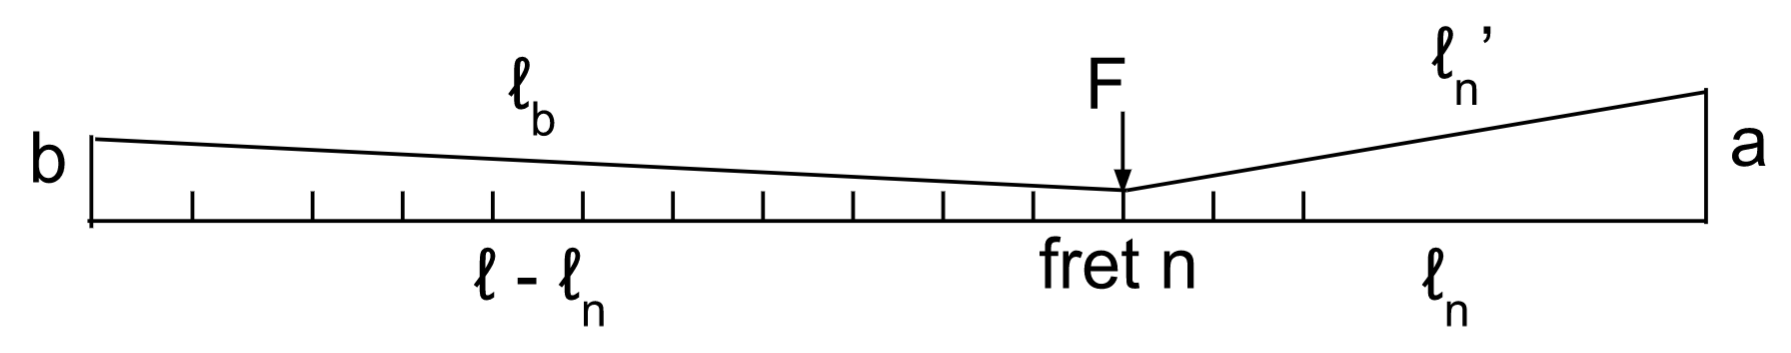
\includegraphics[width=\textwidth]{./ee/fig3.png}
    \caption{A simplified model of the fretted string}\label{fig3}
\end{figure} 

Theoretically, the frequency of this note is 
\begin{equation}\label{eqn5}
    f_n = \frac{1}{2l_n}\sqrt{\frac{T}{\mu}}
\end{equation}

In order to make the frequency match with a specific note in the Western twelve-tone equal temperament (12-TET) system, the scale length needs to be divided into powers of $\sqrt[12]{2}$. To do this luthiers traditionally use a formula to calculate the position of each fret. \cite{eqn6}

\begin{equation}\label{eqn6}
    l_n=\frac{l}{2^\frac{n}{12}}
\end{equation}